%\chapter{Experimental Setup}
\chapter{Setup of Experiments}
\label{chap:experimentalsetup}
\acresetall %reset abbrevations
%\sug{This section describes the experimental setup of the thesis, including details on how the experiments were conducted and evaluated (e.g., evaluation metrics). This section includes the research questions you are aiming to answer, in addition to the hypotheses (if applicable).}
In the following, we detail the experimental setup used to evaluate the performance of the motion models discussed in the preceding chapter. We begin by outlining the central research questions and the specific experiments conducted to address them in Section \ref{sec:rqand}. Subsequently, we describe the unified evaluation framework in Section \ref{sec:evaluationframework}, including the data splits, metrics, and the optimisation and training procedure we employed. Implementation details are described in the last Section \ref{sec:impldetails}.

\ws{Chapter name: Setup of Experiments}
\section{Research Questions and Experiments}
    %\paragraph{Research Questions} 
    \label{sec:rqand}

    The goal of the thesis is to provide a fair comparison between deep learning models, kinematic models, and stochastic filters, and to investigate the impact of incorporating domain information into model training and architecture.
    In particular, the following research questions should be answered: 
    %\todo{what is your new contribution}
    %What specific questions will you answer?
    %Numbered, concrete, answerable questions that your experiments will directly address. Each result chapter should answer at least one.
    \begin{itemize}
      \item \textbf{RQ1:}
      Given a preprocessed dataset and a systematic hyperparameter optimisation procedure, how do deep learning models, both task-specific and pretrained, kinematic baselines, and stochastic filters compare in short-term trajectory prediction of inland vessels?
    
      \item \textbf{RQ2:} 
      %How can information about the vessel’s location (the domain, i.e., lock, harbour, river, channel) be incorporated into motion models, and how does domain-aware modelling affect predictive performance? \sug{bringt diese Information einen Vorteil? wie implementiere ich -> 2 fragen}
    %\todo{new version:}
    Does domain-specific training improve short-term vessel trajectory prediction performance compared to mixed-domain training?
    \end{itemize}
    \vspace{-8pt}
    If \emph{yes}, we investigate encodings of domain knowledge into learned models: \ws{it is not the best to have conditional research questions. Repharse them so that you do not need the "if yes".} \me{I will leave this for now to wait for tims comment. Otherwise, it can simply be left out}
    \begin{itemize}
    \vspace{-8pt}
      \item \textbf{RQ3:} 
     Does adding explicit domain information as one-hot encoded input improve short-term vessel trajectory prediction performance?
    
      %\item \textbf{RQ4:}
     % How well do tuned models generalise when trained and evaluated on a large-scale AIS dataset containing trajectories of thousands of inland vessels? \sug{eigentlcih wird performance schon in frage 1 gemessen. alternative: einfluss der datensetgröße auf performance. braucht neue tests}
    \end{itemize}
%\section{Experimental Setup}
    %\paragraph{Experiments.} 
    %To answer the research questions, we evaluate the selected motion models under a common protocol. %ist jetzt überleitung zu 5.2
    To answer the research questions, we designed three experiments%, referred to as Exp~ \Romannum{1} to  Exp~ \Romannum{3}. They 
    , which differ in the train-test partitioning, the use of domain-specific training, and the use of domain encoding.  %\\        
    
    
        

    
%\todo{hypothese dass wir vermuten pro domäne besser, dann das exp 2.}



        \begin{itemize}
            
        % old title \paragraph{Experiment 0 Mixed Training and Evaluation:} %\me{der title beschreibt was gemacht wird, besser einen titel finden der beschreibt was untersucht wird, also welche frage.}
        \item{\textbf{Exp \Romannum{1}: Baseline Comparison of Motion Models:}} % mixed is implied for Baseline
        Models were trained and evaluated on the full dataset. This Experiment served as the overall comparison across models and model families and aims to answer RQ 1.




        %\paragraph{Experiment 1: Domain specific Training and Evaluation:}
        \item{\textbf{Exp \Romannum{2}: Effect of Domain-Specific Training on Predictive Performance:}}
        Models were trained once separately per domain and once on the mixed dataset. They were then evaluated separately within each domain. This experiment tested whether domain-specific training improves predictive performance compared to mixed-domain training and aims to answer RQ2. 
        % Per-domain training and per-domain evaluation. This tests whether domain-specific training improves performance.
       % Each model is first trained and evaluated separately within every domain.
       % also each model is trained mixed over all domains and evaluated within every domain
       %-> info about domain awareness, model performance, generalisation

         \item{\textbf{Exp \Romannum{3}: Ablation of Explicit Domain Encoding for LSTMs:}}
        
            This study investigated whether explicitly providing domain information as one-hot encoded input improves LSTM performance. To answer RQ3, three LSTM variants were compared under the same data split and evaluation protocol:\begin{itemize}
            \item \textbf{LSTM}: baseline model without domain information.
            \item \textbf{LSTM+Domain}: augments the input with one-hot encoded domain information.
            \item \textbf{LSTM+Domain*}: uses the same architecture as LSTM+Domain but the hyperparameter configuration of the baseline LSTM.
        \end{itemize}
                %In this experiment, we investigate the impact of explicitly encoding domain information into the LSTM architecture.
                %We compare three variants: (i) a plain LSTM baseline, (ii) LSTM + Domain, which , and (iii) LSTM + Domain*, which uses the same architecture as LSTM + Domain %but with the hyperparameter configuration of the baseline LSTM.
               % All models are trained on the full dataset and evaluated on the overall test set as well as separately for the Harbour, River, Channel, and Lock domains using the same train–validation–test splits.
                %We decided not to evaluate on the domain specific sets, since enough insights about domains have been generated in Experiment 2. 
                To assess robustness with respect to random initialisation and non deterministic CUDA training, we additionally trained the baseline LSTM and LSTM + Domain* ten times each with different random seeds, and evaluated the results on the overall test set.
        

        \end{itemize}



\section{Evaluation Framework}%maybe automl in title
\label{sec:evaluationframework}
\ws{This belongs to the experiments chapter. Here only discuss the methods themselves, not how you related evaluate them. The implementations can be kept here, but anything realted to the evaluation (metrics, splitting, .. etc) must be moved to the experiments section}
To systematically execute the experiments outlined above and ensure a fair comparison of prediction quality across all model families, a unified evaluation framework was required.
This section details the shared pipeline we used to perform the comparison.
All experiments utilised the full one-year dataset without downsampling. The data for all experiments were downloaded and preprocessed as described in Chapter~\ref{chap:dataset}.
 Each model received the  normalised feature set 
   % all normalised features it can process
    as a context window and outputs displacement increments $(\Delta x, \Delta y)$. The kinematic models additionally received x and y coordinates as an input, an input we omitted for the deep learning models as per Section \ref{subsec:featureengineering}. %to avoid learning specific trajectories instead of vessel dynamics. 
    The predicted displacements were cumulatively summed and offset by the last known position to reconstruct absolute trajectories before any metric was applied. For testing purposes, both the tuning and evaluation stages support configurable subsampling of data files. \ac{HPO} was performed exclusively on the validation set. The final model and parameters were then evaluated on the test split without retraining.
    

      \subsection{Train-Val-Test Split}
            While formal definitions of the \ac{HPO} and \ac{CASH} problem typically use $k$-fold cross-validation to guide the search \parencite{AutoMLHoos, Feurer2015}, this is mainly designed for traditional machine learning on smaller datasets. For deep learning on our large \ac{AIS} trajectory datasets, we instead used a strict split between training, validation, and test split. In particular, we used a stratified 70:15:15 split, as specified in Section \ref{subsubsec:stratifiedtvtsplit}.  %\\ % for two reasons:
            At the scale of our \ac{AIS} dataset, which can easily be extended with additional recordings of the past years, a single validation set is sufficient to guide hyperparameter search without multiplying training time by $k$. 
            Additionally, we avoided the risk of data leakage by randomly splitting overlapping time series data completely.
            
            %Second, \ac{AIS} trajectories are strongly autocorrelated time series. Randomly splitting individual samples into folds would cause data leakage, since nearby or overlapping trajectory segments from the same vessel could end up in both training and validation. To avoid this, the dataset is split strictly by unique 
            %\texttt{vessel\_id} before segmentation as detailed in %naja mit dem split by vessel id ist es vlt auch möglich, aber so sind wir safe
            %\ref{subsubsec:stratifiedtvtsplit}. This ensures the validation loss $\mathcal{L}$ measures how well the model generalises to completely unseen vessels and gives a realistic picture of its predictive performance.
            

    \subsection{Metrics}
    All trajectory-based metrics were computed from the Euclidean distance between predicted and ground-truth positions. The evaluation was performed over all files in the considered evaluation split and included all predicted time steps, not only the final one, which is separately reflected by the \acf{FDE}. Consistent with common trajectory prediction practice, we additionally reported the \acf{ADE} over all predicted steps and tracks \parencite{donandt2022shortterm, articlebilstmsus}.
    
    In \ac{HPO}, we optimised the \acf{RMSE} of the predicted $x$ and $y$ coordinates. \ac{RMSE} is a standard metric for regression-based prediction tasks and is also used in vessel trajectory prediction by \textcite{articlebilstmsus} and \textcite{donandt2022shortterm} (called $ATE^2$ in the latter). %for the latter
    It was chosen because, due to the squared error term, it penalises large deviations more strongly than absolute-error-based metrics. This is desirable in our setting, where occasional large prediction errors are more problematic than many small ones.
    
    In addition to the aggregated metrics, per-file metrics were computed and stored. % in CSV files. 
    They can serve for further analysis and, in our case, were used for post-hoc statistical tests and to investigate seasonal trends.
    
    Finally, because the foundation models (TiRex and Chronos-2) generate probabilistic quantile forecasts, we employed calibration metrics for their evaluation. Specifically, we assessed the quality of their uncertainty estimates using mean interval width, prediction coverage, and the Winkler score evaluated at the 80\% confidence interval.

    %\paragraph{Statistical tests.} \me{include paragraph in framework section?}
    \subsection{Statistical tests}
    \label{par:statistical}To compare the candidate models statistically, we used the Friedman test followed by a Nemenyi post-hoc test. The Friedman test is a nonparametric alternative to repeated-measures ANOVA and is suitable for comparing multiple models on the same evaluation blocks without assuming normally distributed scores. In our setting, each file served as one block and each model as one treatment. For every file, the models were ranked according to their \ac{RMSE}, with rank 1 assigned to the lowest error. The Friedman test then assessed whether the models differ significantly (\(p < \alpha = 0.05 \)) in their average ranks across blocks.
    
    %\subsection{AutoML Hyperparameter Optimisation} %not entirely accurate with lstm training info dropped in
    \subsection{Optimisation and Training}
    \label{subsec:automlhpo}
    Stochastic filters and deep learning architectures depend on hyperparameter configurations that cannot be easily derived from training data and are impractical to tune manually at scale, since manual tuning risks a biased evaluation, where a model might underperform simply due to a suboptimal configuration rather than an inherent lack of predictive capability.
    To guarantee a fair comparison, each model was optimised independently using \ac{AutoML} in the form of \acf{HPO}. The scope was deliberately restricted to \acs{HPO} rather than the full \ac{CASH} formulation, since domain-specific meta-learning data for a warm start was unavailable: the set of candidate model classes (kinematic models, \acp{KF}, \acp{LSTM}, and foundation models) was chosen manually, while their respective hyperparameters were explored systematically.
    
       % \paragraph{Optimisation Methodology.}

        We centralised the \ac{HPO} for all models. We used the Optuna framework \parencite{optuna_2019}, which supports flexible definition of search spaces, including continuous, integer, and categorical parameters. Optuna was selected because it is easy to set up locally on both Windows and Linux systems, and can be later expanded to be used on a cluster.
        The search for the Deep Learning models was driven by the \acf{TPE}.         
         To optimise computational resources, we employed an early-stopping strategy: an \acs{RMSE}-based callback stopped the search if no improvement greater than a small threshold was observed within a predefined patience window. Also, all tuning experiments were parallelised, with the exception of the Hybrid CV/CTRV, which used the \ac{CV} and \ac{CTRV} models after those were tuned.  %\\
         %Tuning experiments of all models are parallelised.
         To further speed up convergence, we initialised the hyperparameters of the Filters with values found in \ac{HPO} of a small subset of the data. % \me{these werre seeded at random, but i didnt save the seed and didnt save the subset unfortunately}

        \me{this paragraph might as well be part of the lstm implementation details in 5.3.2 below, but also fits here}
         For learned models (\acp{LSTM}), the training procedure during and after \ac{HPO} was as follows.
         We applied pruning using successive halving to reduce total compute: trials were
        evaluated at fixed epoch checkpoints, where only the
        top $1/\eta$ fraction of trials ($\eta = 2$) were allowed to continue,
        while the rest were terminated early. With \texttt{min\_resource} $=8$
        and  \texttt{min\_early\_stopping\_rate} $=0$, the schedule
        evaluated configurations at epochs 8, 16, and 32%, and 64
        . Within each
        surviving trial, an independent early-stopping criterion halted training if
        the validation \ac{RMSE} did not improve by more than
        \texttt{min\_delta} within a fixed patience window.
        To illsutrate these two mechanisms, Figure \ref{fig:succhalfing}. depicts the intermediate validation errors during the \ac{HPO} process of \ac{LSTM} training. It demonstrates how underperforming trials are terminated early at these specific epoch checkpoints and how epochs with little improvement over time are additionally pruned  \me{new, i moved this here from the results. it is more of an illustration than a result}.        
        \begin{figure}[h]
            \centering
            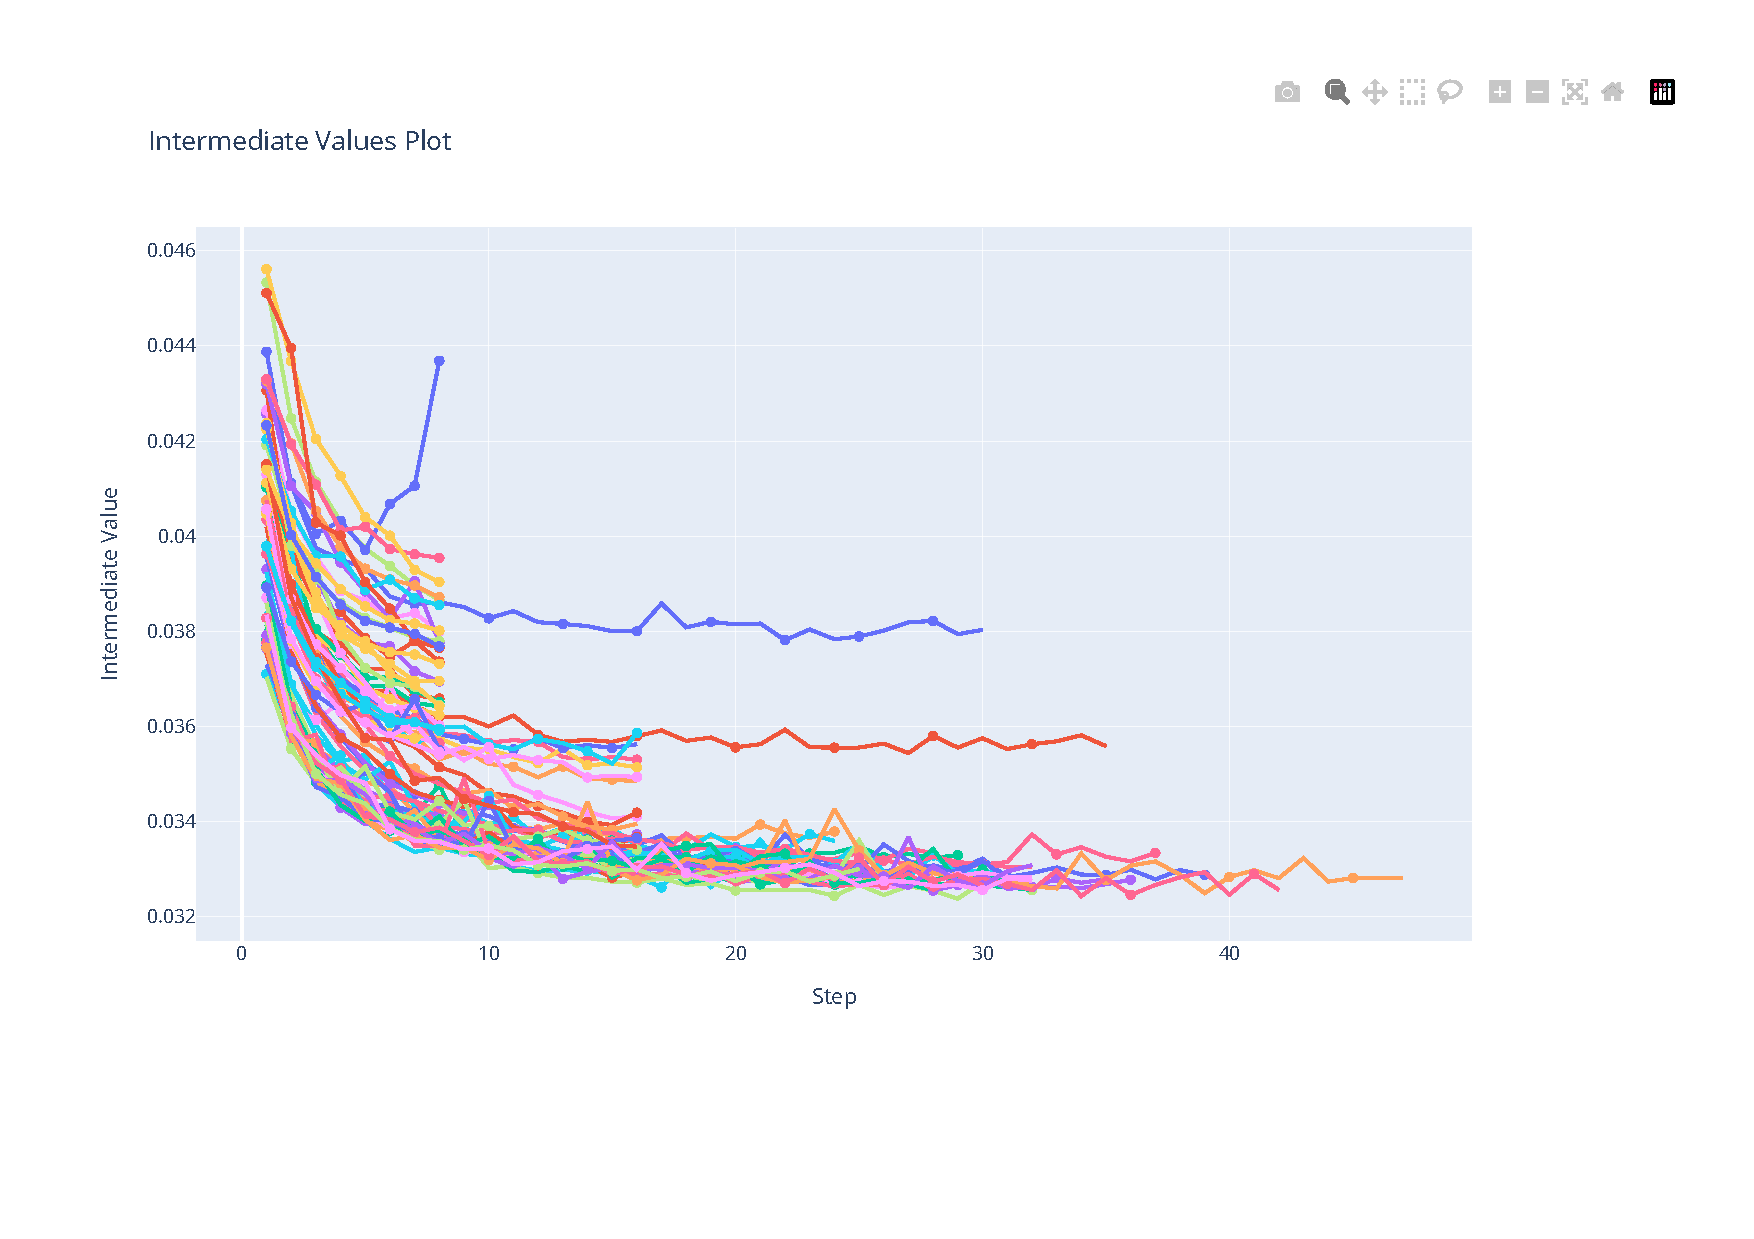
\includegraphics[width=0.9\linewidth,trim=1cm 3.5cm 5.5cm 3.5cm,clip]{figures/minimal_lstm_intermediate_values.html.pdf}
            \caption[Exp. I LSTM Intermediate Value plot]{Intermediate Value plot of \acf{LSTM} \acf{HPO} in Optuna with early stopping enabled. Successive Halving was applied to all trials, except the initial 16. The Drop-offs at stept 8, 16 and 32 indicate points, where the current batch was evaluated and the bottom-performing configurations were terminated}
            \label{fig:succhalfing}
        \end{figure}
        The best-found configuration was retrained from scratch on the full
        training set for up to \texttt{max\_epochs} epochs using the same
        early-stopping criterion, and the resulting checkpoint was used for final
        evaluation on the test split.
        It should be noted that parameter importance scores derived from a pruned
        study are biased towards values that are important early on in the convergence, rather than final validation loss, since most trials do not run to full completion.
         
         Optuna keeps track of intermediate results, enabling us to analyse the learning dynamics after an optimisation run.
          A complete specification of the hyperparameter optimisation methodology and configurations for all experiments is detailed in Table ~\ref{tab:hpo-config} in Appendix \ref{appx:B}.
          Furthermore, the corresponding hyperparameter search spaces for each model are defined within the respective methodology sections (Sections \ref{sec:method-cv} to \ref{sec:method-lstm}) and are additionally summarised in Table \ref{tab:model_hyperparameters} in Appendix \ref{appx:B}.



                
        \paragraph{Search Spaces and Strategies.}
        The optimisation strategy varies according to the complexity of the model:
        \begin{itemize}
            \item \textbf{Kinematic Models:} These models contain small, 1-Dimensional search spaces. We employed a full grid search over all valid configurations to ensure the global optimum for these parameters was found.  \ac{TPE} with n trials $\gg$ valid configurations can also find the global optimum, but comes with a computational overhead we wanted to avoid. For fairness, we only used the validation split for this optimisation, ignoring the test split.
            \item \textbf{Filters:} We mapped the Covariance and Uncertainty matrices to a multi-dimensional continuous search space using log-uniform distributions, as the optimal values typically span several orders of magnitude. The search was then guided using \ac{TPE}.
            \item \textbf{Foundation Models:} Chronos is designed as a pure Zero-Shot model and requires no \ac{HPO}. For TiREX, we optimised the size of the input window analogously to the kinematic models, since the model does not implement any attention mechanisms.
            \item \textbf{Learned Sequence Models:} These models involve higher-dimensional parameter spaces. We used \acs{TPE} to navigate the search space.

        \end{itemize}
            
           \paragraph{Feature Selection.} 
           \label{subsub:featureselection}
        
           Within the optimisation process of our models, we treated the input feature subset as a categorical hyperparameter. Rather than relying on manual feature ablation, the selection of which \ac{AIS} signals to include is then integrated directly into the search space. This reflects prior research showing that optimal feature subsets and model hyperparameters are interdependent, as the best configuration for one inherently depends on the other \parencite{Feurer2015}.
           The automated selection was not used for univariate models (TiREX), where other channels cannot influence performance, and models that implement attention across channels (Chronos-2), since those already autonomously identify the most relevant contributions during training and make explicit feature search redundant.                 
           %Absolute $x,y$ positions are strictly excluded from the search space of the deep-learning models to force them to learn generalizable vessel dynamics rather than location-specific patterns. \me{zum dritten.. am ende schauen was wo steht und dann halt nur das erste behalten}
        To make sure that all 16 candidate feature sets were covered at least once in model training of the \acs{LSTM}, one trial was enqueued to the study for each candidate. Those trials were identical, except for the feature set. After that, 10 additional startup trials were sampled uniformly at random %to seed the surrogate        model 
        before the optimisation began. The full search space for the \acp{LSTM} is listed
        in Table~\ref{tab:lstm-hpo}. 


        
                          
     \begin{table}[t]
        
        \centering
        \begin{tabular}{lll}
        \toprule
        \textbf{Hyperparameter} & \textbf{Type} & \textbf{Values / Range} \\
        \midrule
        \texttt{hidden\_size}   & Categorical & $\{64, 128, 256\}$ \\
        \texttt{num\_layers}    & Fixed       & $2$ \\
        \texttt{dropout}        & Continuous  & $[0.1,\, 0.4]$ (uniform) \\
        \texttt{learning\_rate} & Continuous  & $[10^{-4},\, 10^{-2}]$ (log-uniform) \\
        \texttt{batch\_size}    & Categorical & $\{128, 256, 512\}$ \\
        %\texttt{feature\_set}   & Categorical & $\{dx\_norm, dy\_norm\} \cup \mathcal{P}\big(\{ \{cog\_sin\_norm, cog\_cos\_norm\}, sog\_norm, rot\_norm \}\big)$ \\
        \texttt{feature\_set} & Categorical & %$\{dx\_norm, dy\_norm \cup S \}$ \\
        $\{\texttt{dx\_norm},\, \texttt{dy\_norm}\} \cup S$ \\
        \bottomrule
        \end{tabular}
        \\ with $S \in \mathcal{P}(\{\{cog\_sin\_norm, cog\_cos\_norm\}, sog\_norm, rot\_norm, dt\_norm\})$
        \caption[LSTM Hyperparameter Search Space]{Hyperparameter search space used for the \ac{LSTM} model optimization. Continuous parameters are sampled from uniform or log-uniform distributions, categorical parameters are selected from predefined sets. For the \texttt{feature\_set}, The base input always includes $\texttt{dx\_norm, dy\_norm}$. The remaining features are drawn from the power set $\mathcal{P}$ of $\{\{\texttt{cog\_sin\_norm}, \texttt{cog\_cos\_norm}\}, \texttt{sog\_norm}, \texttt{rot\_norm}, \texttt{dt\_norm}\}$, where sine and cosine of \acf{COG} are treated as an indivisible pair 
        \me{We always take dx and dy as an input. for all other inputs, we take all possible combinations of these, with the restriction of sine and cosine of cog only appearing together. since power sets are not applied recursively, this notation seems complicated, but is unambiguous. or did i make a mistake?}}
        \label{tab:lstm-hpo}

        \end{table}   
        


\section{Implementation Details}
\label{sec:impldetails}
\me{i moved this full section into the experimental setup. all general information is included in the methdos section}

    %\subsection{Sequence Model Implementation}%the ones i chose in chapter 2 
    \label{sec:sequenceimplementation}
    In this section, we describe the sequence models we have selected for vessel trajectory prediction and how they were implemented. Two categories were evaluated: foundation models applied zero-shot, and \ac{LSTM} models trained on the full dataset.      
        \subsection{Foundation Models} %some points double with the Framwwork chapter, but i feel like they belong in both. e.g. the zero shot evaluation and hpo. here it i smore detailed
        \paragraph{TiRex.}
        \textcite{auer2025tirexzeroshotforecastinglongtrex} designed TiRex as a Univariate Zero-Shot Forecaster that leverages the new scaling capabilities of the \ac{x-LSTM}.
        Our implementation is characterised by:
        \begin{enumerate}
            \item Univariate channels: To predict $dx, dy$, we fed the model only with the normalised $dx\_norm$, $dy\_norm$, which the model treats independently.
            \item Zero-Shot Evaluation: We used the Model as is. Because no attention mechanisms is implemented, we optimised only the input length. Due to the univariate character, feature selection was not a factor in our optimisation.
            %\item Probabilistic Modelling: TiRex generates quantile forecasts for the prediction horizon. %In this implementation, we use the quantiles 0.1 and 0.9.  to evaluate uncertainty via interval width, coverage,  and Winkler score. % \me{nur auf nachfrage näher drauf eingehen, denke das kennt man} \
            %\me{move evaluation} \todo!
        \end{enumerate}
        

        
        \paragraph{Chronos-2.}
         
        % https://proceedings.mlr.press/v162/ozturk22a/ozturk22a.pdf ) for weights no HPO
        In addition to the univariate TiRex, we implemented Chronos-2 \parencite{ansari2025chronos2} as a zero shot transformer for time series forecasting. Unlike the \ac{LSTM} based model, it lacks the inductive bias for time series. Instead, it supports Co-variate informed forecasting.  %\\%unrelated
        The model was designed to estimate a probability distribution over future trajectories rather than computing a deterministic path. Our implementation is characterised by:
    
        \begin{enumerate}
            \item Multivariate Covariates: To predict $dx, dy$, we fed the model with all available normalised features: $sog\_norm$, $cog\_sin\_norm$, $cog\_cos\_norm$, $dt\_norm$, $rot\_norm$  as covariates, in addition to the $dx\_norm$, $dy\_norm$ channels.
            \item Zero-Shot Evaluation: We used the Model as is, without doing any \ac{HPO} or finetuning. To avoid overhead, we deliberately did not add the feature selection to our \ac{HPO}, since we can assume, that the cross-channel attention of Chronos-2 already gives low weights to irrelevant features. %\me{siehe comments}%\ref{fig:platzhalter_test_channel_importance_chronos2_zero_shot.png} assumption bestätigen in auswertung \cite{someone to undermine this is good methodology}. 
            For a similar reason, the context length was set to the maximum 10 steps available after preprocessing, as the self attention implemented in the transformer can recognise irrelevant timestamps. %\ref{figplatzhalter_ gleichemitzeit}
            %\item Probabilistic Modelling: Chronos-2 generates quantile forecasts for the prediction horizon. In this implementation, we use the quantiles 0.1, 0.5, and 0.9. The median $q_{0.5}$ is used as the point forecast. The remaining quantiles are used to evaluate uncertainty via interval width, coverage, % CRPS approximation, and Winkler score. % \me{nur auf nachfrage näher drauf eingehen, denke das kennt man}
        \end{enumerate}
    
    
        \begin{comment}

        Beyond our standard metrics, we compute the%two scores post-hoc:
        %\textbf{Channel Importance}. This analysis ranks the predictive information of input features. For each covariate, the Pearson correlation between the feature values and the vessel's movement is computed. The resulting absolute correlations are normalised to provide a relative importance score for each input channel.
        \textbf{Channel Importance}. This analysis quantifies the linear association between each input feature and the vessel's motion magnitude. For each covariate, the absolute Pearson correlation with the motion magnitude is computed across all samples, then normalised by the sum of all absolute correlations to yield a relative importance score for each input channel.
        \textbf{Timestep Importance}. This analysis quantifies the linear association between each context timestep's motion magnitude and the future motion score. For each timestep in the context window, the absolute Pearson correlation with the future motion score is computed across all tracks, then normalised by the sum of all absolute correlations to yield a relative importance score per timestep. If all correlations are zero, uniform weights are assigned.
                
        \textbf{Timestep Importance}. This analysis quantifies the model’s temporal sensitivity. It computes the correlation between the movement at each context step and the future motion. The resulting scores reveal the model's "attention" distribution.
        \me{please tell me if this makes sense, the plots show nearly no difference except for lock, which might make sense}
        \me{scrapped, still in the code though. Actually results make sense becuse ofr lock its differnt as we are standing first. but metric was too ambigious and hard to explain}


        weggelassen weil: 
        The importance is computed from the correlation between input covariates and motion magnitude in the data  not from anything the model does internally. Both Chronos and LSTM evaluate on the same tracks with the same input features, so the Pearson correlations are identical. The model is irrelevant to the calculation.

        \end{comment}


    \subsection{LSTM} %im vergleich zu den vorherigen liest sich das etwas holprig
    \label{sec:method-lstm}
  
    
    The \ac{LSTM} represents learned sequence models in our comparison.
    Unlike the kinematic models and filters, which encode an explicit motion
    assumption, the \ac{LSTM} can learn temporal dynamics directly from the data.
    Unlike the foundation models, it was trained from scratch on the \ac{AIS}
    dataset, giving full control over architecture, feature set, and training
    procedure.
    \ws{do not mention training detials here. This belongs o the experiments section.}
    
        \paragraph{Architecture.}

        The model follows a \ac{Seq2Seq} %sequence-to-sequence 
        \ws{you have this as ac} 
        encoder--decoder design
        (Figure~\ref{fig:mylstm}): a stacked \ac{LSTM} encoder
        processes the context window and compresses it into a hidden state, which
        seeds the decoder. The decoder then predicts all future displacements simultaneously. We picked the linear prediction instead of an autoregressive decoder, due to the faster compute time.
        \ws{These are all experiment-related details, not method-sepcific.        Example, instead of writing how many layers you picked in the experiments, here you can write about the LSTM AE can have multiple stacked layers in general.} 
        % and its better suitability for short prediction horizons \me{source}.
        
        %an autoregressive decoder. \todo{design decision} The decoder predicts one displacement
        %step $(\hat{\Delta x}, \hat{\Delta y})$ at a time, feeding each prediction
        %back as the next input for up to $T_p$ steps.
        
        %The absolute trajectory is then reconstructed by cumulative summation of the displacements, offset by the last known position, as described in Section~\ref{sec:evaluation-framework}.
        The number of layers was fixed at 2 to keep the search space reasonable. Dropout was applied between layers for regularisation. More more details about the feature selection can be found in Section \ref{subsub:featureselection}. 
        \begin{figure} [h]
            \centering
            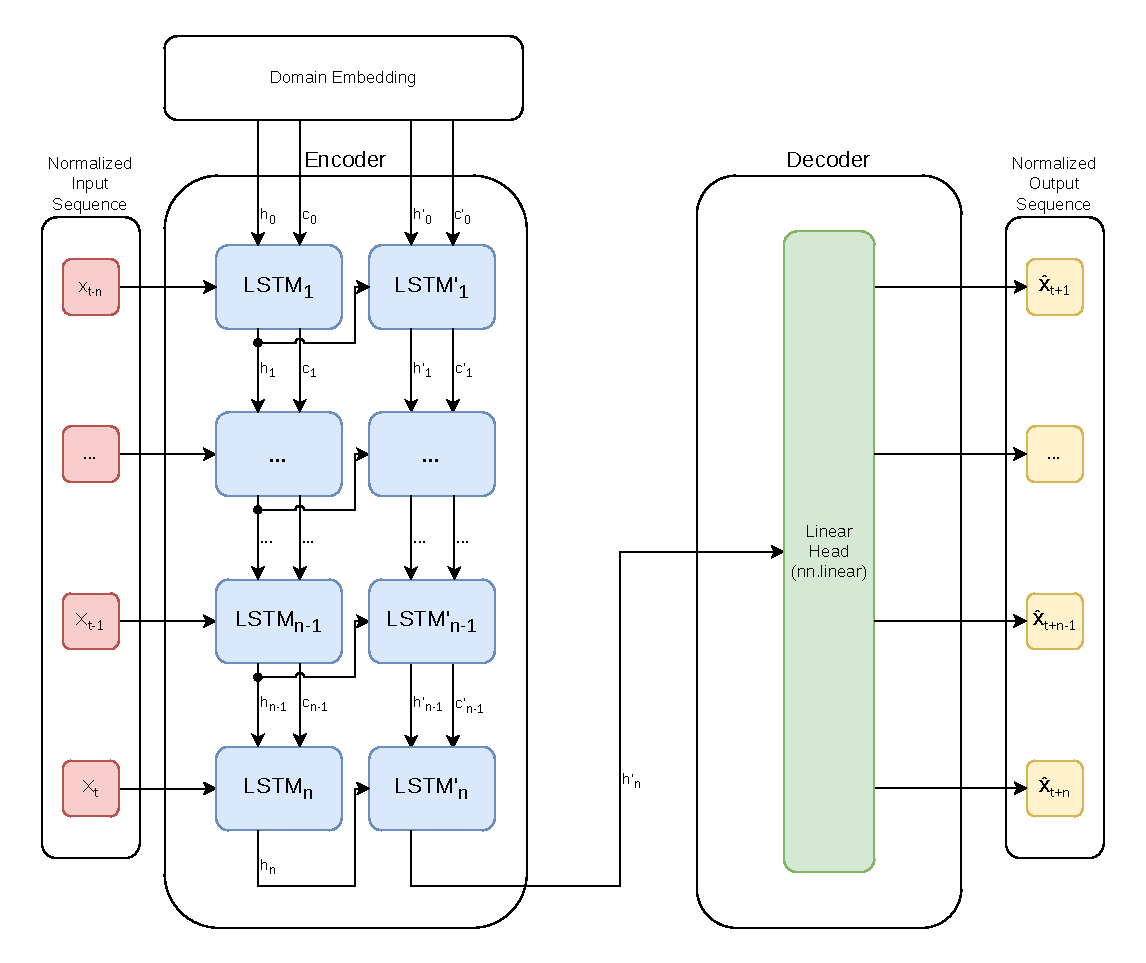
\includegraphics[width=0.85\linewidth]{figures/MyLSTM.drawio.pdf}
            \caption[Proposed LSTM Architecture]{The \acf{LSTM} Architecture implemented in this work: 2 \ac{LSTM} Encoding Layers feed into a Linear Decoder. The Initial Cell and Hidden state are initialised with the Embedded Domain. The figure is self-made.}
            \label{fig:mylstm}
        \end{figure}
        %\paragraph{Feature Selection.}
%Eigentlich alles redundant mit Evaluation Framework
        %\me{unsure if the followiong 2 sentences should be removed}
        \ws{Replace with: more details about the hyperparameters are in Seciton xxx}
        %As described in \ref{subsub:featureselection}, feature selection from our feature candidates is handled using categorical hyperparameters. We suggested \(sog\_norm\), \(cog\_sin\_norm\), \(cog\_cos\_norm\), \(dt\_norm\), \(rot\_norm\) as covariates, in addition to the \(dx\_norm\) and \(dy\_norm\) channels.
        
        % \(dx\_norm\), \(dy\_norm\) are always included, \(cog\_sin\_norm\), \(cog\_cos\_norm\) optionally included as a set, as well as \(sog\_norm\), \(rot\_norm\) and \(dt\_norm\)  as optional features.

        %Since this approach exploded the search space, we only ran it on a sampled 30\% of the total Training and validation set, and then continued training with the selected feature set. The optimisation picked the full feature set as the best candidate. OUTDATED
        %/home/dustin_klein/motion-models/output/08_baseline_results/runs/lstm_30_full_categorical/tuning/optuna_plots only on request

        %To make sure that every set of features is evaluated, we initially run one trial per feature set with a fixed set of hyperparameters, before further optimizing with \ac{TPE}.

        \ws{The follwing has a lot of details that is specific to you experimetns, here you only mention the methods and their implementations in general without the details specific to your experiments}
        \paragraph{Domain Encoding.}
        In the \textit{\ac{LSTM} + domain} variant, the domain is represented as a 4-dimensional one-hot encoded vector, with one dimension per class. Instead of appending the domain vector as an input feature at every timestep, it is added to the initial hidden and cell states of both LSTM layers. Specifically, the last 4 nodes of the initial hidden state $h_0$ and cell state $c_0$ are set to the one-hot vector. The remaining nodes are initialised to zero as usual. This keeps the total hidden size identical to the baseline model and ensures a fair comparison.  %\\
        Encoding the domain only in the initial states is acceptable here, since we focus on short term predictions and only need to retain the contextual information over 10 timesteps. %\\
        We considered adding additional groupings for domains with similar expected behaviours or constraints, but decided against this in order to avoid introducing potentially incorrect assumptions about the domain structure.
       
        A learned embedding layer was considered as an alternative. However, for only four domain classes, one-hot encoding is preferable as it is parameter-free, exact, and directly interpretable. In contrast, learned embeddings introduce additional trainable parameters and reduce interpretability, since the resulting coordinates no longer correspond directly to individual domain classes. This trade-off is usually more attractive for higher-cardinality categorical variables; if the number of domains were to grow substantially in future work, an embedding-based representation could become worth it.

        
        %\paragraph{Hyperparameter Optimisation.} \me{probably also move this into the setu of experiments}

        %The hyperparameter search space for the \ac{LSTM} is summarised in Table~\ref{tab:lstm-hpo}. The optimisation methodology, including the pruning schedule and trial budget, is detailed in Section \todo{move and reference}.
    
    \begin{comment}
             Hyperparameters are tuned using \ac{TPE} via Optuna \parencite{optuna_2019}, minimising \ac{RMSE} on the validation split.
            To make sure they are all covered at least once, for each of the 16 candidate feature sets, one trial is enqueued to the study. Those trials are identical, exept for the feature set. After that, 10 additional startup trials are sampled uniformly at random %to seed the surrogate        model 
            before the optimisation begins. The full search space is listed
            in Table~\ref{tab:lstm-hpo}. 
            
                  
            
            Pruning using successive halving is applied to reduce total compute: trials are
            evaluated at fixed epoch checkpoints, where only the
            top $1/\eta$ fraction of trials ($\eta = 2$) is allowed to continue,
            while the rest are terminated early. With \texttt{min\_resource}$\,=8$
            and \texttt{min\_early\_stopping\_rate}$\,=0$, the schedule
            evaluates configurations at epochs 8, 16, 32, and 64. Within each
            surviving trial, an independent early-stopping criterion halts training if
            the validation \ac{RMSE} does not improve by more than
            \texttt{min\_delta} within a fixed patience window.
                   
            It should be noted that parameter importance scores derived from a pruned
            study are biased towards values that are important early on in the convergence, rather than final
            validation loss, since most trials do not run to full completion.
            
            The best-found configuration is retrained from scratch on the full
            training set for up to \texttt{max\_epochs} epochs using the same
            early-stopping criterion, and the resulting checkpoint is used for final
            evaluation on the test split.
    
        
   

\begin{table}[t]
        \caption[LSTM hyperparameter search space]{Hyperparameter search space used for the \ac{LSTM} model optimization. Continuous parameters are sampled from uniform or log-uniform distributions, categorical parameters are selected from predefined sets. For the \texttt{feature\_set}, the model always receives normalized positional displacements, combined with a subset $S$ drawn from the power set $\mathcal{P}$ of the remaining kinematic and temporal features: $\{\{\texttt{cog\_sin\_norm}, \texttt{cog\_cos\_norm}\}, \texttt{sog\_norm}, \texttt{rot\_norm}, \texttt{dt\_norm}\}$. \me{not sure how to explain this compactly for the table. We always take dx and dy as an input. for all other inputs, we take all possible combinations of these, with the restriction of sine and cosine of cog only appearing together}}
        \label{tab:lstm-hpo}
        \centering
        \begin{tabular}{lll}
        \toprule
        \textbf{Hyperparameter} & \textbf{Type} & \textbf{Values / Range} \\
        \midrule
        \texttt{hidden\_size}   & Categorical & $\{64, 128, 256\}$ \\
        \texttt{num\_layers}    & Fixed       & $2$ \\
        \texttt{dropout}        & Continuous  & $[0.1,\, 0.4]$ (uniform) \\
        \texttt{learning\_rate} & Continuous  & $[10^{-4},\, 10^{-2}]$ (log-uniform) \\
        \texttt{batch\_size}    & Categorical & $\{128, 256, 512\}$ \\
        %\texttt{feature\_set}   & Categorical & $\{dx\_norm, dy\_norm\} \cup \mathcal{P}\big(\{ \{cog\_sin\_norm, cog\_cos\_norm\}, sog\_norm, rot\_norm \}\big)$ \\
        \texttt{feature\_set} & Categorical & $\{\{dx\_norm, dy\_norm\} \cup S \}$ \\
        \bottomrule
        \end{tabular}
        \end{table}
        with $S \in \mathcal{P}(\{\{cog\_sin\_norm, cog\_cos\_norm\}, sog\_norm, rot\_norm, dt\_norm\})$

        \end{comment}
